\section{Hyperparameter Search}

% \begin{frame}
% % \frametitle{Hyperparameter Search}
% \only<1>{
%     \begin{figure}
%         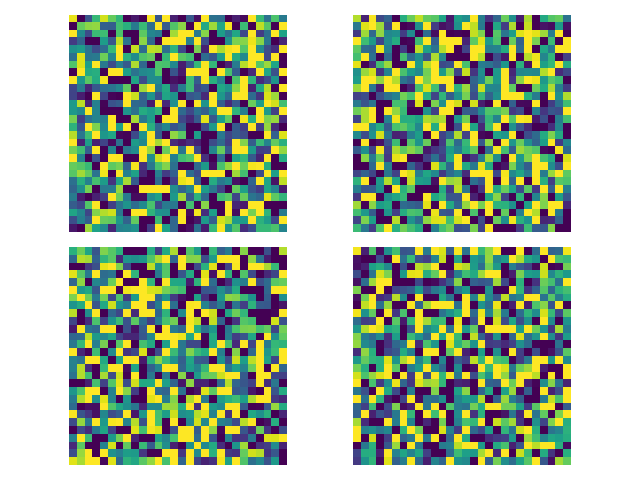
\includegraphics[width=0.7\textwidth]{images/randomMemories/05.png}
%     \caption{\(n=20\)}
%     \end{figure}
% }
% \only<2>{
%     \begin{figure}
%         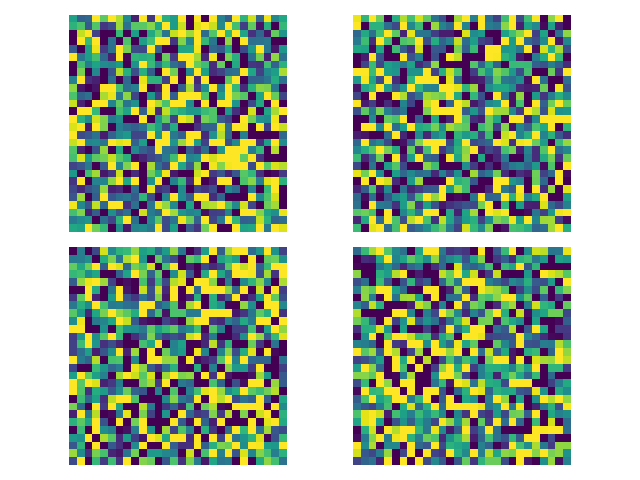
\includegraphics[width=0.7\textwidth]{images/randomMemories/06.png}
%     \caption{\(n=15\), \(\beta=600\)}
%     \end{figure}
% }
% \only<3>{
%     \begin{figure}
%         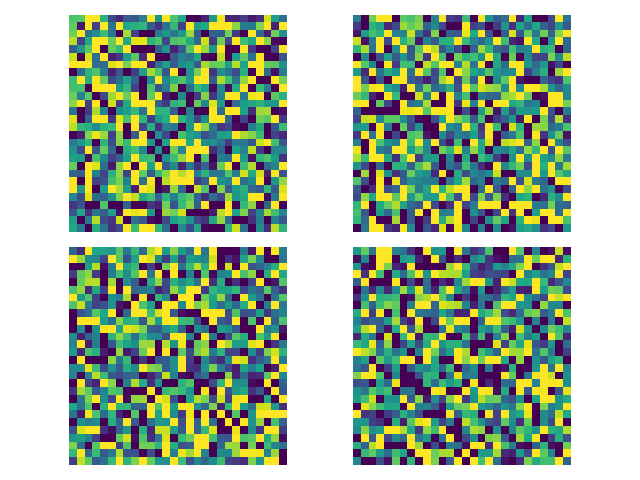
\includegraphics[width=0.7\textwidth]{images/randomMemories/07.png}
%     \caption{\(n=12\), \(\beta=545\), \(\text{lr}=0.01\)}
%     \end{figure}
% }
% \only<4>{
%     \begin{figure}
%         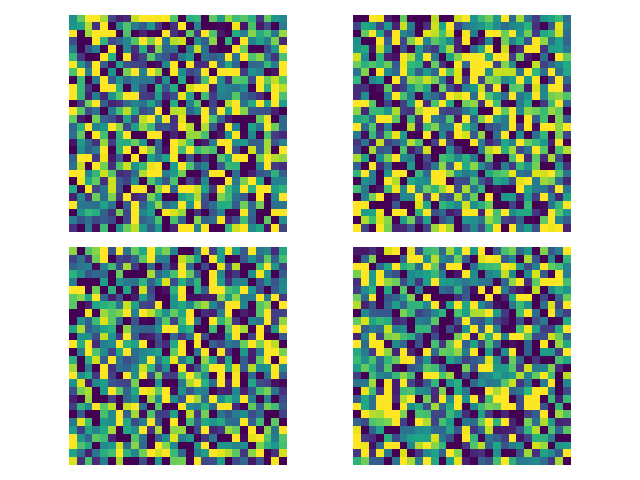
\includegraphics[width=0.7\textwidth]{images/randomMemories/08.png}
%     \caption{\(n=17\), \(\beta=730\), \(\text{lr}=1.0\), \(\text{lr}_\text{decay}=0.99\)}
%     \end{figure}
% }
% \only<5>{
%     \begin{figure}
%         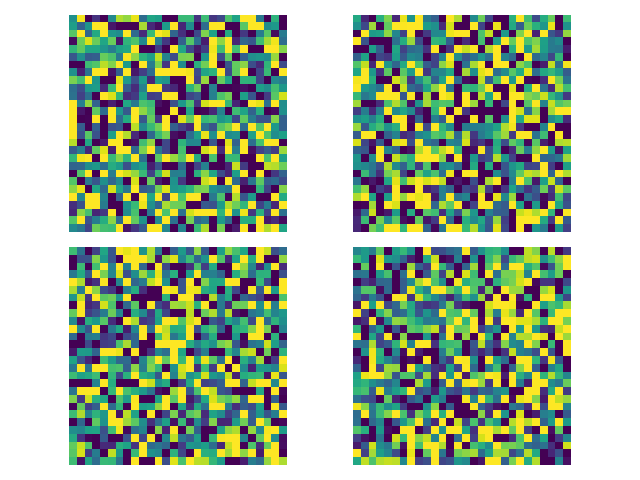
\includegraphics[width=0.7\textwidth]{images/randomMemories/09.png}
%     \caption{\(n=30\), \(\beta_i=700\), \(\beta_f=500\), \(\text{lr}=1.0\), \(\text{lr}_\text{decay}=0.99\), Interaction Function=Leaky Rectified Polynomial, \(\text{Momentum}=0.6\), \(\text{Error Power}=2\)}
%     \end{figure}
% }
% \end{frame}

%------------------------------------------------

\begin{frame}
    \frametitle{Hyperparameter Search}
    Training our network on autoassociative tasks of dimension 100. \\

    We measure the Euclidean distance between learned state and recalled state. Lower is better, as this corresponds to a well recalled memory.
\end{frame}

%------------------------------------------------

\begin{frame}
    \frametitle{Hyperparameter Search: \(n=2\)}

    \begin{figure}
        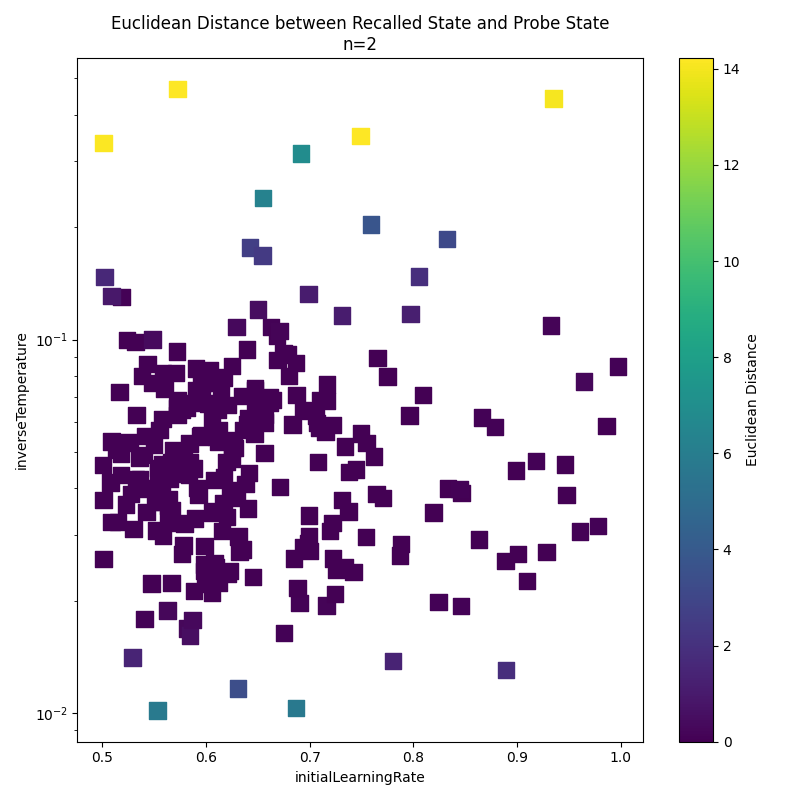
\includegraphics[width=0.6\textwidth]{images/initialHyperparameterSearches/2.png}
    \end{figure}
    % TODO: Ellipse to show what is "good" region?
\end{frame}

\begin{frame}
    \frametitle{Hyperparameter Search: \(n=3\)}

    \begin{figure}
        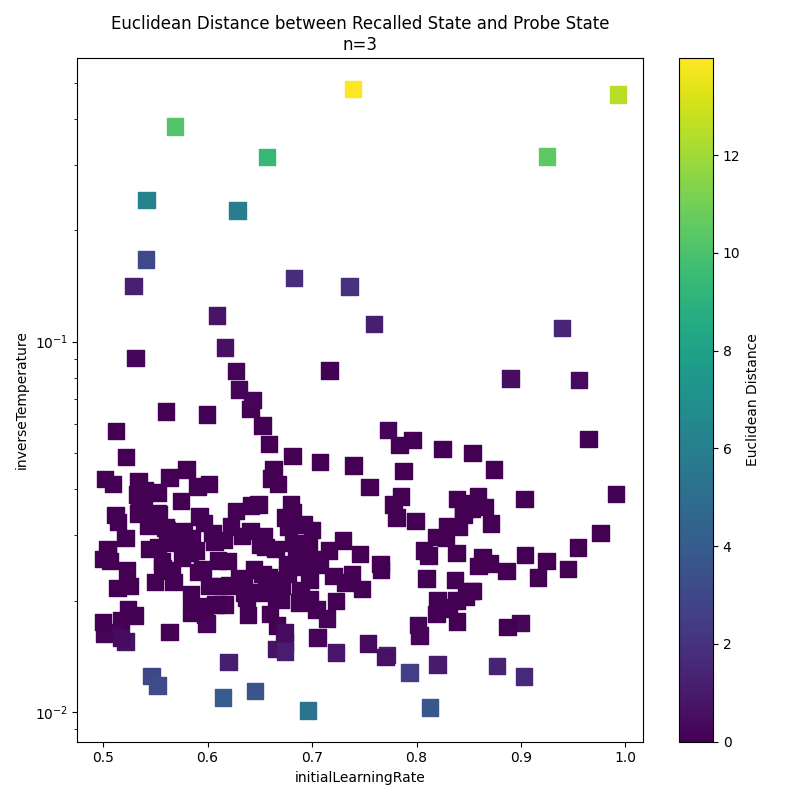
\includegraphics[width=0.6\textwidth]{images/initialHyperparameterSearches/3.png}
    \end{figure}
\end{frame}

\begin{frame}
    \frametitle{Hyperparameter Search: \(n=5\)}

    \begin{figure}
        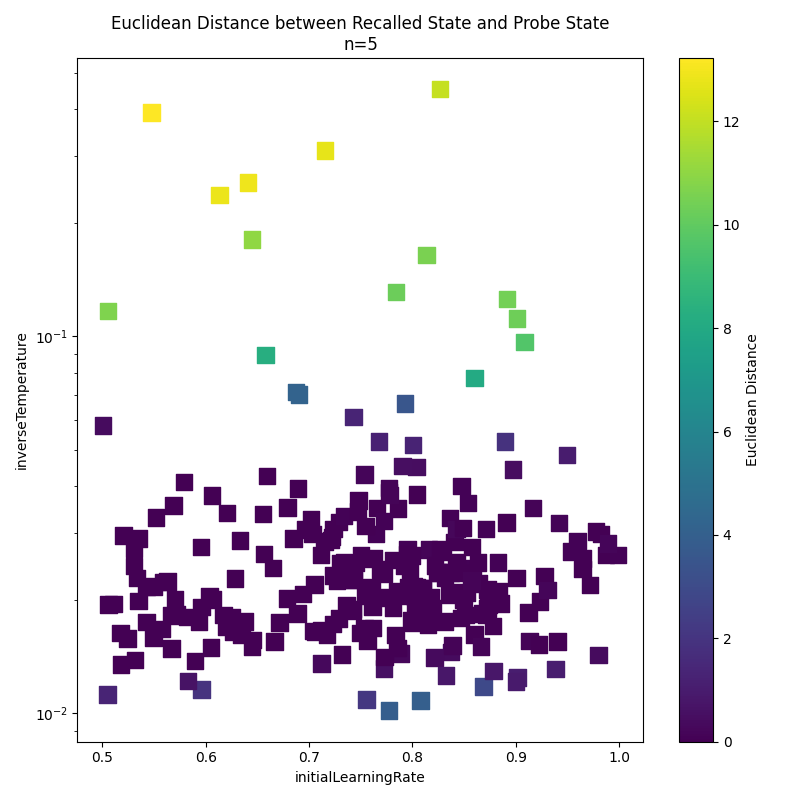
\includegraphics[width=0.6\textwidth]{images/initialHyperparameterSearches/5.png}
    \end{figure}
\end{frame}

\begin{frame}
    \frametitle{Hyperparameter Search: \(n=10\)}

    \begin{figure}
        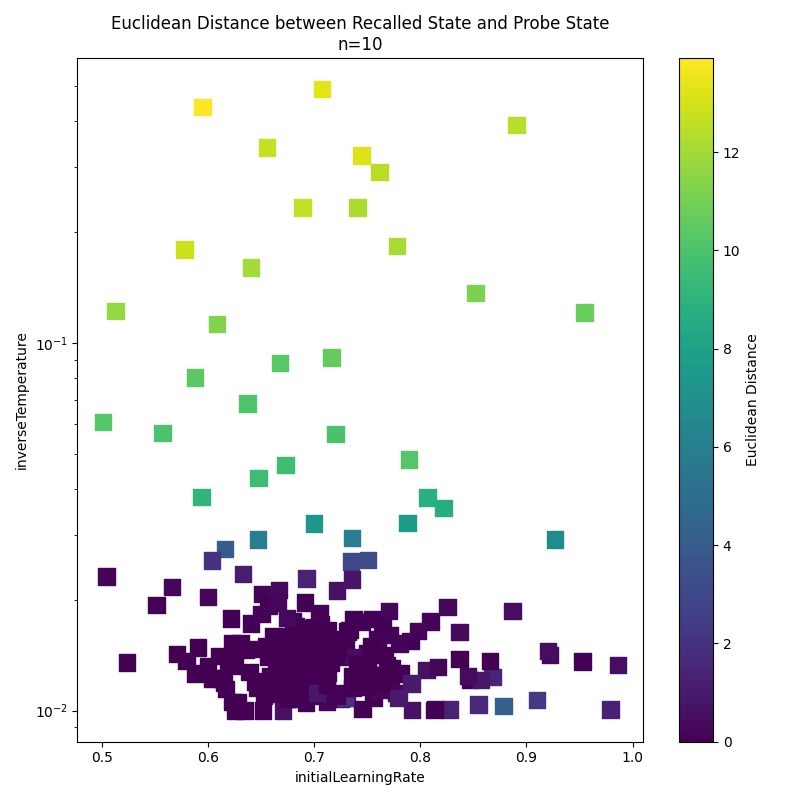
\includegraphics[width=0.6\textwidth]{images/initialHyperparameterSearches/10.png}
    \end{figure}
\end{frame}

\begin{frame}
    \frametitle{Hyperparameter Search: \(n=15\)}

    \begin{figure}
        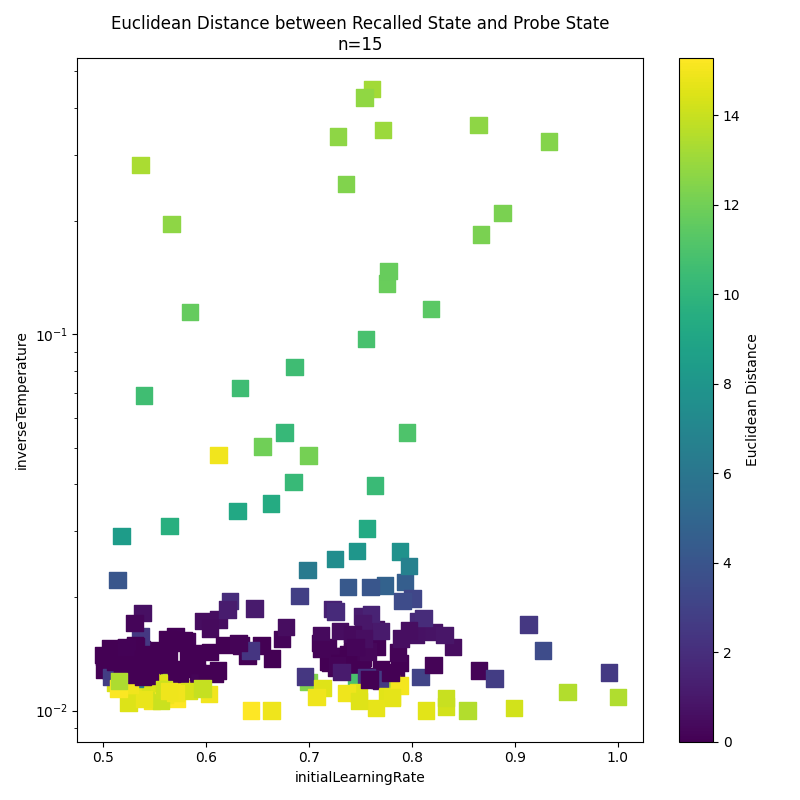
\includegraphics[width=0.6\textwidth]{images/initialHyperparameterSearches/15.png}
    \end{figure}
\end{frame}

\begin{frame}
    \frametitle{Hyperparameter Search: \(n=20\)}

    \begin{figure}
        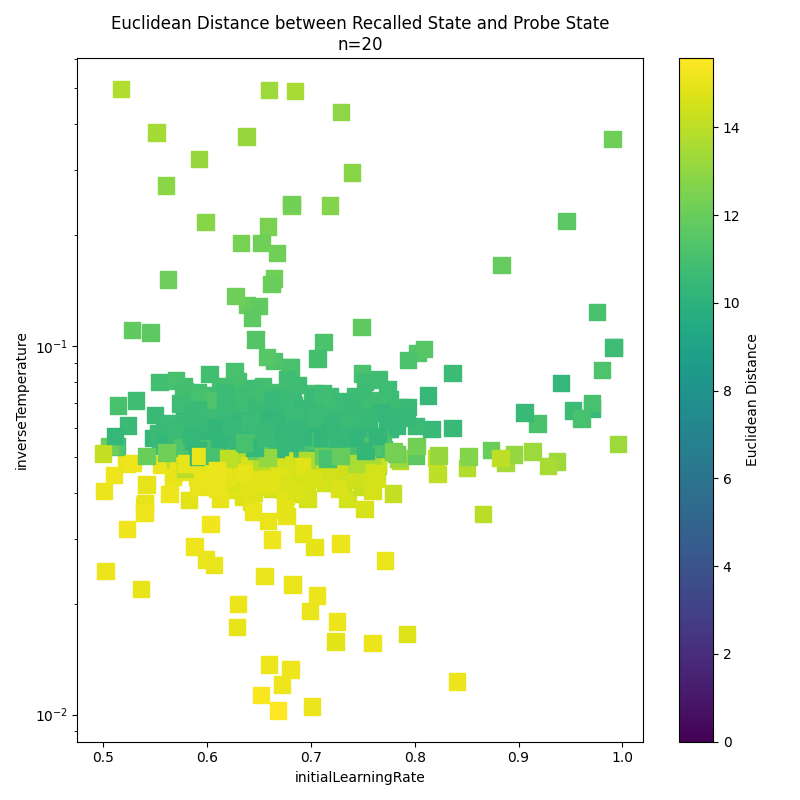
\includegraphics[width=0.6\textwidth]{images/initialHyperparameterSearches/20.png}
    \end{figure}
\end{frame}

\begin{frame}
    \frametitle{Hyperparameter Search: \(n=25\)}

    \begin{figure}
        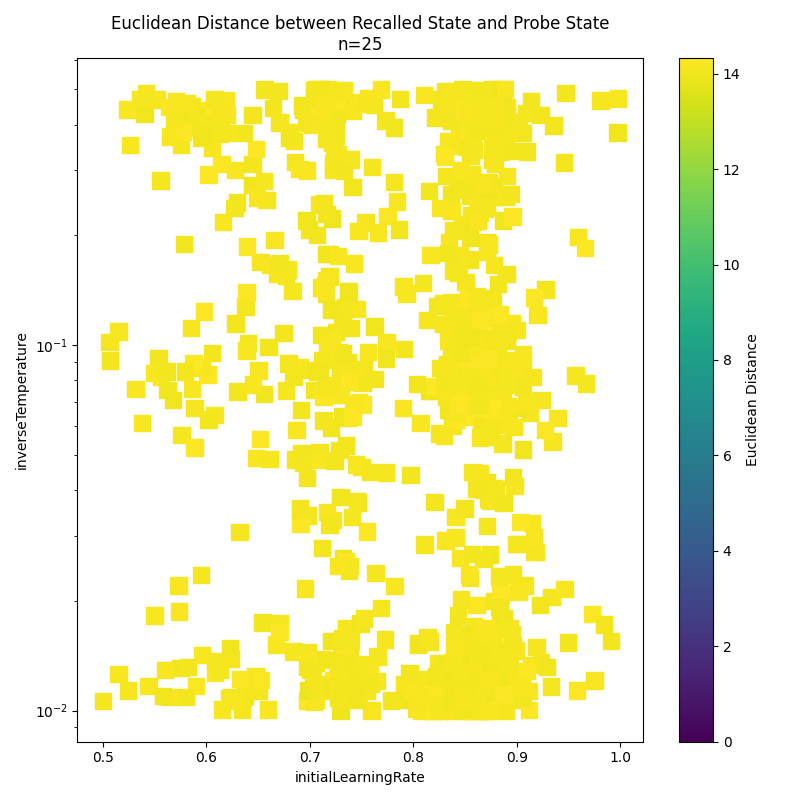
\includegraphics[width=0.6\textwidth]{images/initialHyperparameterSearches/25.png}
    \end{figure}
\end{frame}

%------------------------------------------------